\documentclass{beamer}
\usetheme{Madrid}

\usepackage{amsmath}
\usepackage{graphicx}

\usepackage{tikz}

\usepackage[justification=centering]{caption}
\usepackage{subcaption}

\usepackage{xurl}

% default path to images and other assets
\graphicspath{{assets/}}

% disable wrapping
\tolerance=1
\emergencystretch=\maxdimen
\hyphenpenalty=10000
\hbadness=10000

% number figure caption
\setbeamertemplate{caption}[numbered]

% display bib label in references
\setbeamertemplate{bibliography item}{\insertbiblabel}
\setbeamertemplate{bibliography entry title}{}
\setbeamertemplate{bibliography entry location}{}
\setbeamertemplate{bibliography entry note}{}

% Metadata
% ------------------------
\title[Instance segmentation]{Instance segmentation of biomedical images with an object-aware
embedding learned with local constraints}
\subtitle{Seminar Computational Life Science}

\author[Oleh Shkalikov]{Oleh Shkalikov \texorpdfstring{\\ 5102818}{}}

\institute[TU Dresden]{TU Dresden, Computer Science Faculty}

\date{9 May, 2023}

% ------------------------

\begin{document}

\frame{\titlepage}

\begin{frame}
    \frametitle{Agenda}
    \tableofcontents
\end{frame}

\section{Problem formulation}

\begin{frame}
    \frametitle{Instance Segmentation}

\end{frame}

\begin{frame}
    \frametitle{Semantic VS Instance Segmentation}

    \begin{figure}[h]
        \begin{subfigure}{0.5\textwidth}
            \centering
            \includegraphics[width=0.95\textwidth]{semantic_segm_example.png}
            \caption{Semantic segmentation}
        \end{subfigure}
        \begin{subfigure}{0.49\textwidth}
            \centering
            \includegraphics[width=0.95\textwidth]{instance_segm_example.png}
            \caption{Instance segmentation}
        \end{subfigure}
        \caption{Comparison of the different segmentation types. Source publication is \cite{segm_type_comp}}.
    \end{figure}

\end{frame}

\begin{frame}
    \frametitle{Metric}

\end{frame}

\section{Previous approaches}

\begin{frame}
    \frametitle{Approaches to Solve the Problem}

    \centering
    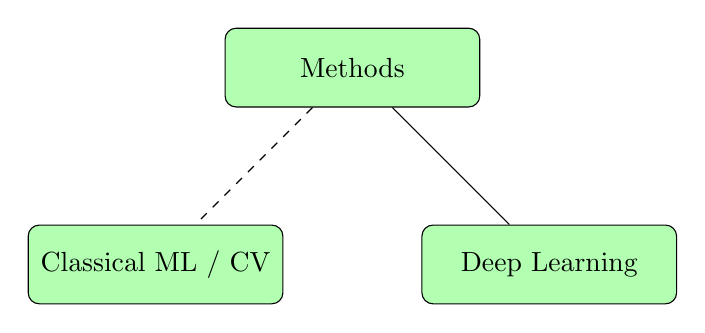
\begin{tikzpicture}[nodes={rectangle, rounded corners, minimum width=3cm, text width=3cm, minimum height=1cm,text centered, draw=black, fill=green!30},
            sibling distance=5cm, level distance=2.5cm]
        \node {Methods}
        child {node(a){Classical ML / CV} edge from parent [dashed]}
        child {node(b){Deep Learning}};
    \end{tikzpicture}

    \vspace*{0.5cm}
    \begin{block}{Why Deep Learning?}
        Neural networks significantly outperforms all classical
        methods because they can be represented as a learnable feature
        extractor and regressor or classification head. Whereas classical approaches are
        based on hand-made or fixed features which are hard to derive and not flexible.
    \end{block}

\end{frame}

\begin{frame}
    \frametitle{Neural Network Building Blocks}

    \begin{figure}[h]
        \begin{subfigure}[t]{0.5\textwidth}
            \centering
            \includegraphics[width=0.85\textwidth]{conv2d.pdf}
            \caption{Padded 2D Convolution. Source: \cite{zhang2021dive}}
        \end{subfigure}
        \begin{subfigure}[t]{0.49\textwidth}
            \centering
            \includegraphics[width=0.8\textwidth]{pooling.pdf}
            \caption{Max Pooling. Source: \cite{zhang2021dive}}
        \end{subfigure}
        \begin{subfigure}{0.5\textwidth}
            \centering
            \includegraphics[width=0.8\textwidth]{upsampling.png}
            \caption{Nearest Neighbour Upsampling. Source: \cite{phdthesis}}
        \end{subfigure}
        \begin{subfigure}{0.49\textwidth}
            \centering
            \includegraphics[width=0.9\textwidth]{dropout.pdf}
            \caption{Dropout (1 dim case). Source: \cite{zhang2021dive}}
        \end{subfigure}
        \caption{Basic building blocks of CNNs}.
    \end{figure}

\end{frame}

\begin{frame}
    \frametitle{UNet}

    \begin{figure}[h]
        \includegraphics[width=0.8\textwidth]{unet.png}
        \caption{Original UNet architecture from \cite{ronneberger2015u}}
    \end{figure}

\end{frame}

\begin{frame}
    \frametitle{Mask R-CNN}

    \begin{block}{Two stage}
        Mask R-CNN is a two stage architecture: region proposal
        and classification with segmentation / bounding box refinement.
    \end{block}

    \begin{figure}[h]
        \begin{subfigure}{0.65\textwidth}
            \includegraphics[width=\textwidth]{mask_rcnn.png}
            \caption{Mask R-CNN pipeline}
        \end{subfigure}
        \begin{subfigure}{0.34\textwidth}
            \includegraphics[width=\textwidth]{roi_align.png}
            \caption{ROI align}
        \end{subfigure}
        \caption{Mask R-CNN architecture \cite{he2017mask}}
    \end{figure}

\end{frame}

\begin{frame}
    \frametitle{Stardist}

    \begin{block}{Idea of Stardist}
        A model is trained to densely predict the distances ($r$)
        to the object boundary \textbf{along a fixed set of rays} and object
        probabilities ($d$), which together produce an
        overcomplete set of candidate polygons for a given
        input image. The final result is obtained via
        non-maximum suppression of these candidates.
    \end{block}

    \begin{figure}[h]
        \includegraphics[width=\textwidth]{stardist.png}
        \caption{Stardist explanation. Source: \cite{schmidt2018}}
    \end{figure}

\end{frame}

\begin{frame}
    \frametitle{Previous Works Summary}

    \begin{itemize}[<+->]
        \item Sematic segmentation based method predicts contours $\implies$
              few misclassified pixel ends up with one big connected region crowded objects
        \item Approaches which are using NMS, like Mask R-CNN, suppress objects when their bounding boxes
              overlap with a large ratio
        \item Stardist is suitable only for fixed shape objects
    \end{itemize}

\end{frame}

\section{Proposed method}

\begin{frame}
    \frametitle{Network architecture}

    \begin{block}{Idea}
        Compute pixel-wise embeddings which will be similar within the
        object but orthogonal for every two \textbf{neighboring} objects.
    \end{block}

\end{frame}

\begin{frame}
    \frametitle{Actual Implementation}


\end{frame}

\begin{frame}
    \frametitle{Loss function}



\end{frame}

\begin{frame}
    \frametitle{Postprocessing}



\end{frame}

\section{Analysis of the performance}

\begin{frame}
    \frametitle{Qualitative results }



\end{frame}

\begin{frame}
    \frametitle{Cell Dataset Metrics}



\end{frame}

\begin{frame}
    \frametitle{Leaf Dataset Metrics}



\end{frame}

\section{Further researches}

\begin{frame}
    \frametitle{Instance Segmentation of Dense and Overlapping Objects via Layering}



\end{frame}

\begin{frame}
    \frametitle{SOTA in the Instance Segmentation}

\end{frame}

\section*{Conclusions}
\begin{frame}
    \frametitle{Conclusions}



\end{frame}

\section*{References}

\begin{frame}[allowframebreaks]
    \frametitle{References}

    \nocite{chen2019instance}

    \bibliographystyle{apalike}
    \bibliography{references.bib}
\end{frame}

\end{document}